\documentclass[11pt, oneside]{article}

\usepackage{geometry}            
\geometry{letterpaper}
\usepackage{graphicx}
\usepackage{caption}
\usepackage{authblk}
\usepackage{amssymb}
\usepackage{pst-node}
\usepackage{tikz-cd} 
\usepackage{tikz}
\usepackage{amsmath}
\usepackage{verbatim}
\usepackage{subfig}
\usetikzlibrary{positioning}
\usepackage{hyperref}
\usepackage{authblk}
\usepackage{float}
\newcommand{\verbatimfont}[1]{\renewcommand{\verbatim@font}{\ttfamily#1}}

\makeatletter
\g@addto@macro\@floatboxreset\centering
\makeatother

\graphicspath{ {../src/images/}{./images} }

\title{Image Analysis and Computer Vision Homework}
\author{Giorgio Romeo}
\affil{Politecnico di Milano \\ A.Y. 2021/2022}
%\date{}							% Activate to display a given date or no date


\begin{document}
\maketitle

\begin{figure*}[!b]
	\centering
	
\includegraphics[width=0.7\linewidth]{Logo_Politecnico_Milano.png}
	\label{logo}
\end{figure*}

\pagebreak
\tableofcontents
\pagebreak

\section{Introduction}
The homework is based on the back side of Villa Melzi d’Eril in Bellagio. In the bottom view below (Fig. \ref{scene}), all lines lie on a same horizontal plane $\Pi$. In addition the facades 1 and 5 are coplanar, and both are parallel to facade 3. Furthermore, facades 2 and 4 are perpendicular to facades 1, 3 and 5. The sun is placed at the point at the infinity
$ S = [3.9\quad \text{-} 1\quad z\quad 0]^\intercal $
-where $z$ is irrelevant- with respect to to the reference frame reported in the picture. The layout of the architectonic elements on facade 3 is symmetric with respect to a central vertical axis. Windows of facades 1, 3 and 5 are are equally wide. Windows of facades 2 and 4 can not be exploited in reconstruction since they are poorly visible.

An image of the back side of Villa Melzi d’Eril is taken by a digital camera (Fig. \ref{Villa}). The camera skew factor is assumed to be null; the aspect ratio is unknown (thus natural camera can not be assumed), as well as the principal point and the focal distance. The camera height (z-coordinate) over the ground plane is 1.5 m.\\


\begin{figure}[!h]
\centering
\begin{minipage}{.5\textwidth}
	\centering
	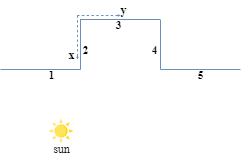
\includegraphics[width=1\linewidth]{scene.png}
	\captionof{figure}{Scene}
	\label{scene}
\end{minipage}%
\begin{minipage}{.5\textwidth}
	\centering
	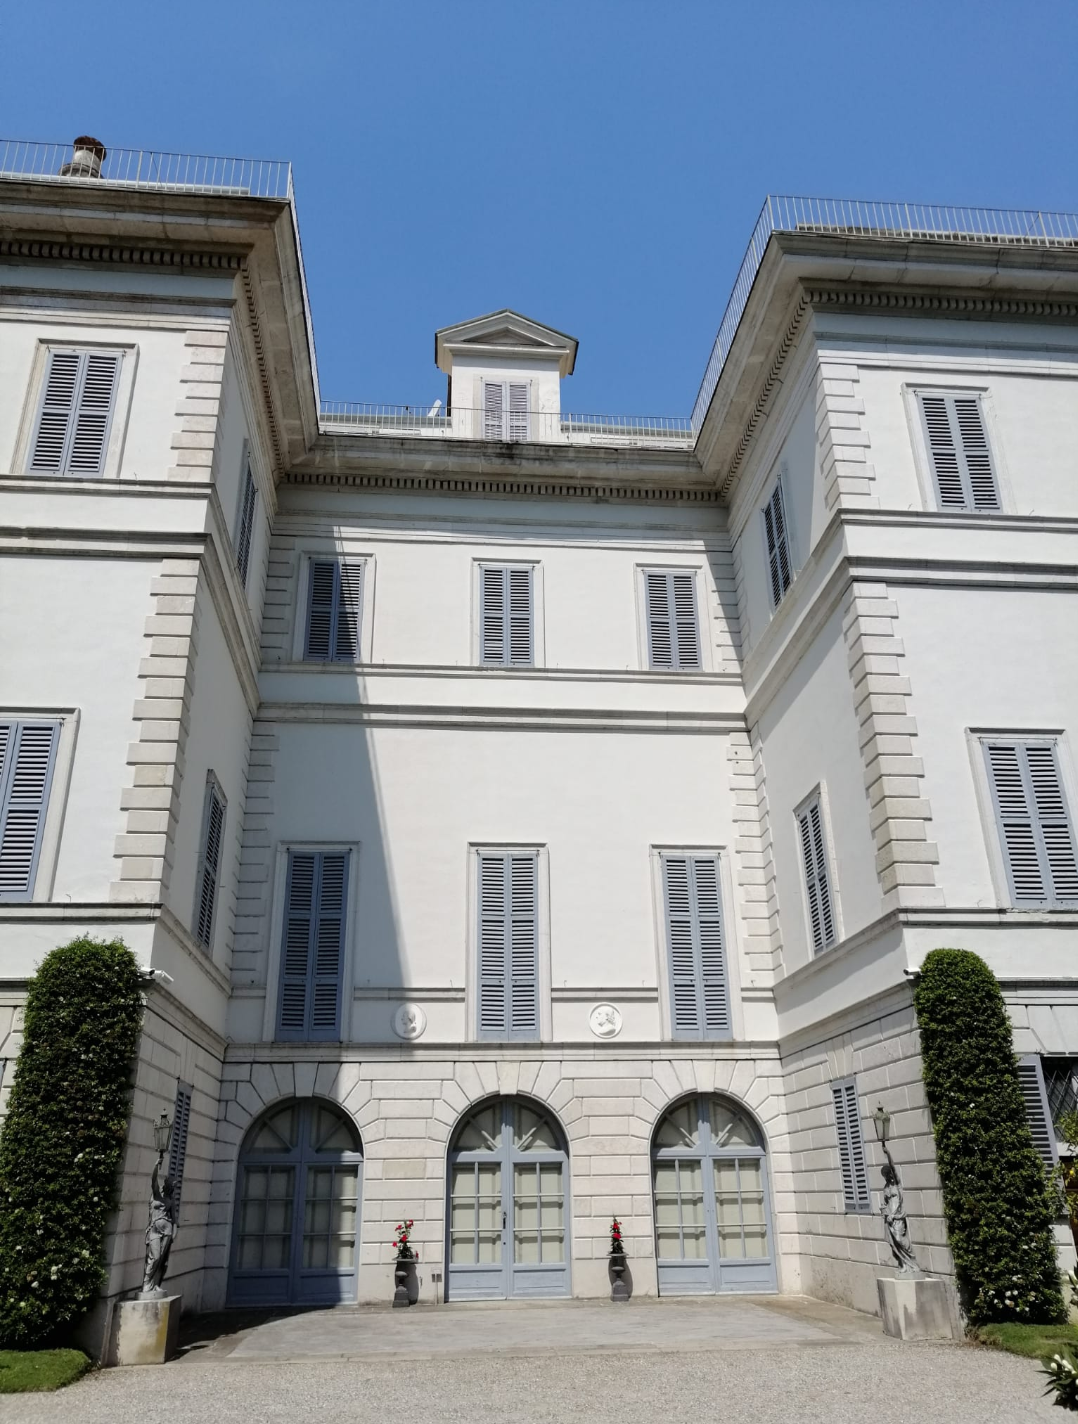
\includegraphics[width=0.5\linewidth]{Villa.png}
	\captionof{figure}{Back side of Villa Melzi d'Eril}
	\label{Villa}
\end{minipage}
\end{figure}


\section{Feature extraction}
\textbf{Combining the learned techniques, find edges, corner features and straight lines in the image.} \hfill \break
The features were extracted in three steps:
\begin{itemize}
	\item Edge detection using Canny algorithm
	\item Line detection using Hough transform
	\item Corner detection using Harris-Stevens algorithm
	
\end{itemize}

\subsection{Edge detection}
The Canny algorithm relies on a multi-stage edge detector. It can be divided in three steps:
\begin{itemize}
	\item \textit{Computation of the magnitude and angle of the directional gradients}: it uses a filter based on the derivative of a Gaussian in order to compute the intensity of the gradients. The Gaussian reduces the effect of noise present in the image.
	\item \textit{Non-Maximum suppression}: the image magnitude produces results in thick edges but the final image should have thin edges. Thus, to thin out the edges, we perform non-maximum suppression by finding the pixel with the maximum value in an edge
	\item \textit{Hysteresis thresholding}: some edges may not actually be edges and there is some noise in the image. Double thresholding deals with this problem. A pixel is considered an \textit{edge pixel} if its gradient is above "high" threshold, a \textit{non-edge pixel} if its gradient is below "low" threshold. Furthermore, if the gradient at a pixel is between "low" and "high" thresholds then declare it an edge pixel if and only if it can be directly connected to an edge pixel or connected via pixels between "low" and "high".
\end{itemize}
The threshold parameters found for Canny algorithm are the result of many experiments. Note that the line extraction part is affected by this final result.
The processed image with extracted edges is shown in figure \ref{image_edges}.
\begin{figure*}[!h]
	\centering
	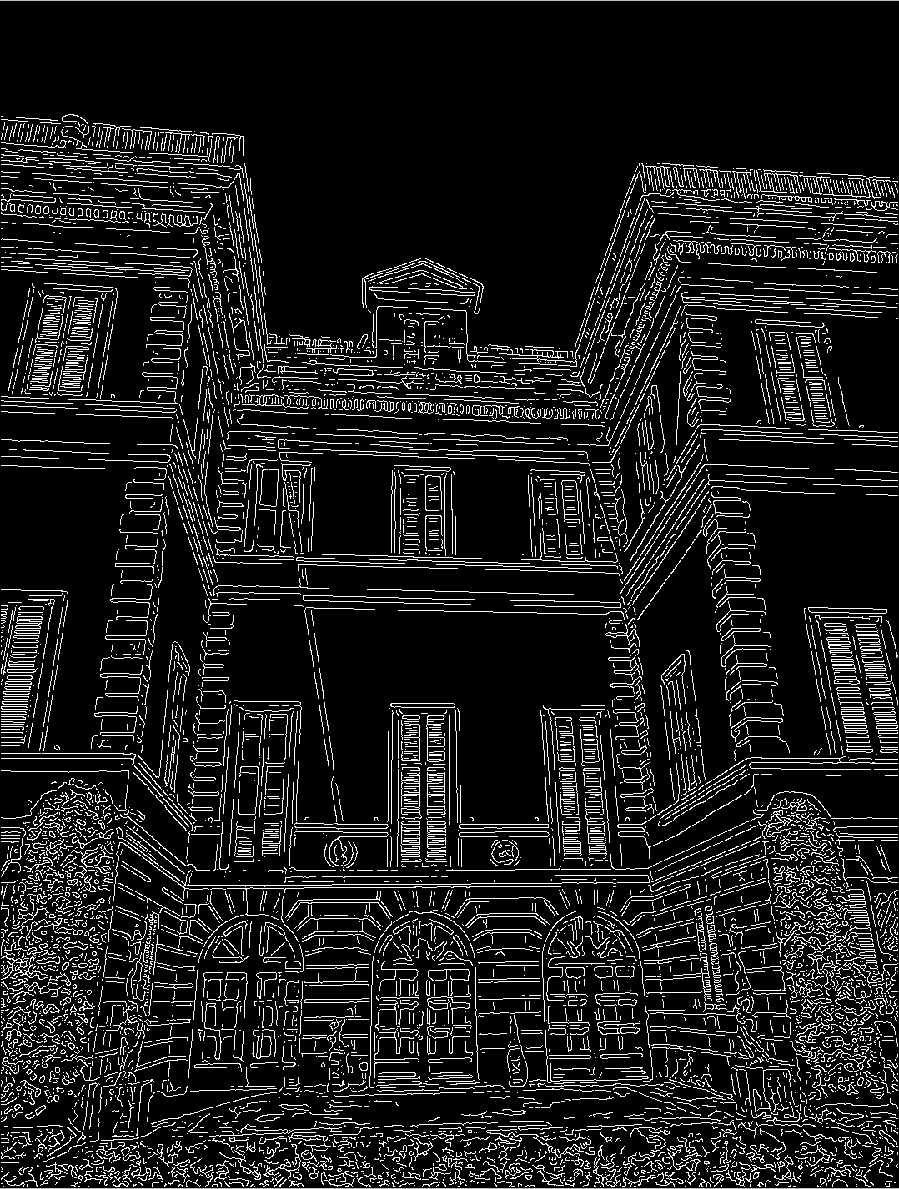
\includegraphics[width=0.43\linewidth]{image_edges.png}
	\captionof{figure}{Extracted edges of the image}
	\label{image_edges}
\end{figure*}

\subsection{Line detection}
The Hough transform is a technique that can be used to isolate features of a particular shape within an image. In our case, the Hough transform is used to detect straight lines. Since the Cartesian representation for lines does not include vertical lines, it is more convenient to utilize the parametric notation:
$ rho = x*cos(\theta) + y*sin(\theta) $.

Each datum (edge point extracted using Canny algorithm) votes for all models compatible with it. The steps followed are:
\begin{itemize}
	\item Discretization of the Hough Space into cells
	\item For each cell, set a vote counter equals to 0
	\item For each datum:
		\begin{itemize}
			\item Compute the Hough Transform
			\item Determine cells crossed by Hough Transform
			\item Increment vote counter for crossed cells
		\end{itemize}
	\item Select cells where vote counter is greater than a threshold and is a local max
	\item Refine line estimate by refitting to points that voted that line
\end{itemize}
The result of the application of the Hough Transform for line detection is shown in Fig. \ref{image_lines}.
\begin{figure*}[!h]
	\centering
	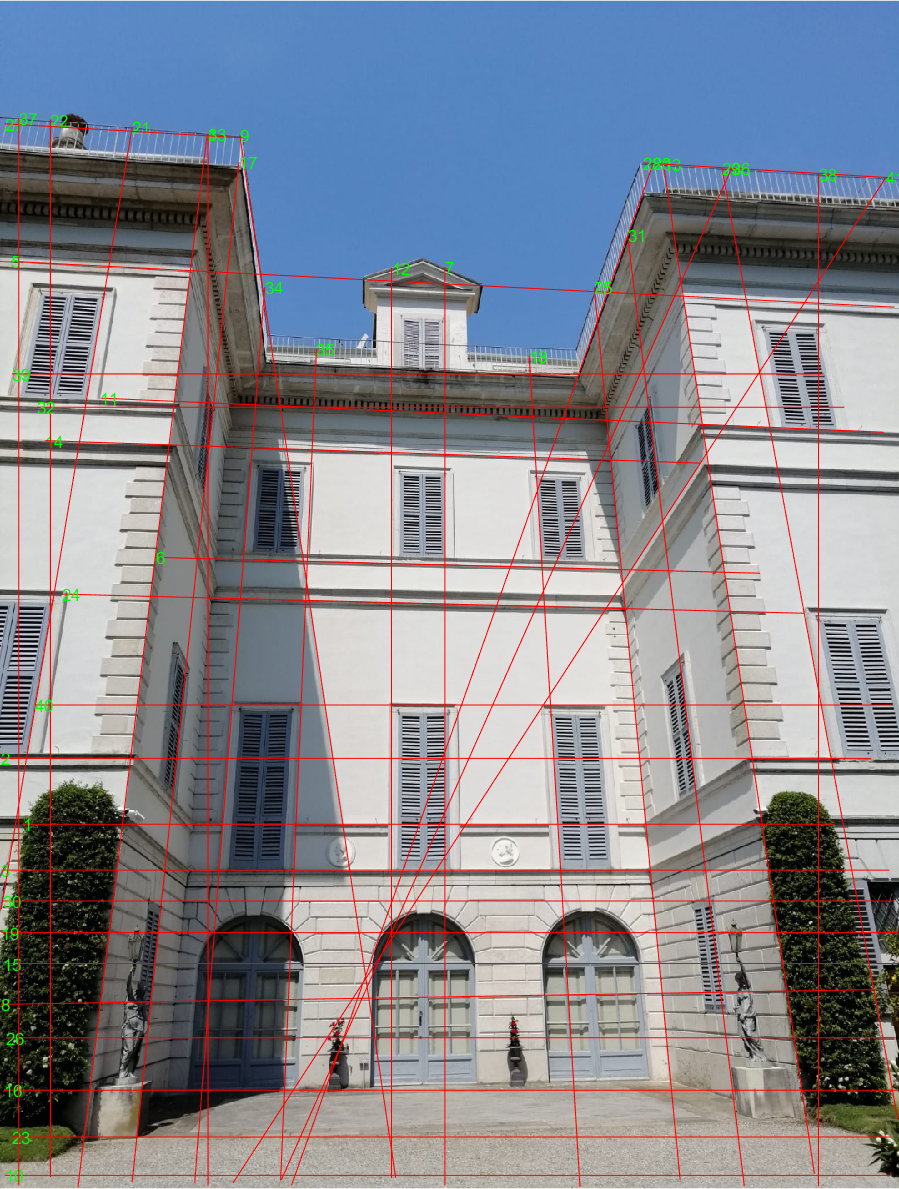
\includegraphics[width=0.3766\linewidth]{image_lines.png}
	\captionof{figure}{Extracted lines of the image}
	\label{image_lines}
\end{figure*}


\subsection{Corner detection}
A corner can be interpreted as the junction of two edges, where an edge is a sudden change in image brightness. Harris-Stevens algorithm considers a small window (in our case 3 x 3) around each pixel in the image. We want to identify all pixel windows that are unique, where uniqueness can be measured by shifting each window by a small amount in a given direction and measuring the amount of change that occurs in the pixel values.

We compute the sum squared difference (SSD) of the pixel values before and after the shift and identify pixel windows where the SSD is large for shifts in all 8 directions. We define the change function E(u,v) as the sum of all the SSD, where u,v are the x,y coordinates of every pixel in our 3 x 3 window and I is the intensity value of the pixel. The features in the image are all pixels that have large values of E(u,v) with respect to a pre-defined threshold. The algorithm identifies a corner if the SSD is be large in shifts for all eight directions.

The processed image with extracted corners is shown in figure \ref{image_corners}.\\
\begin{figure*}[!h]
	\centering
	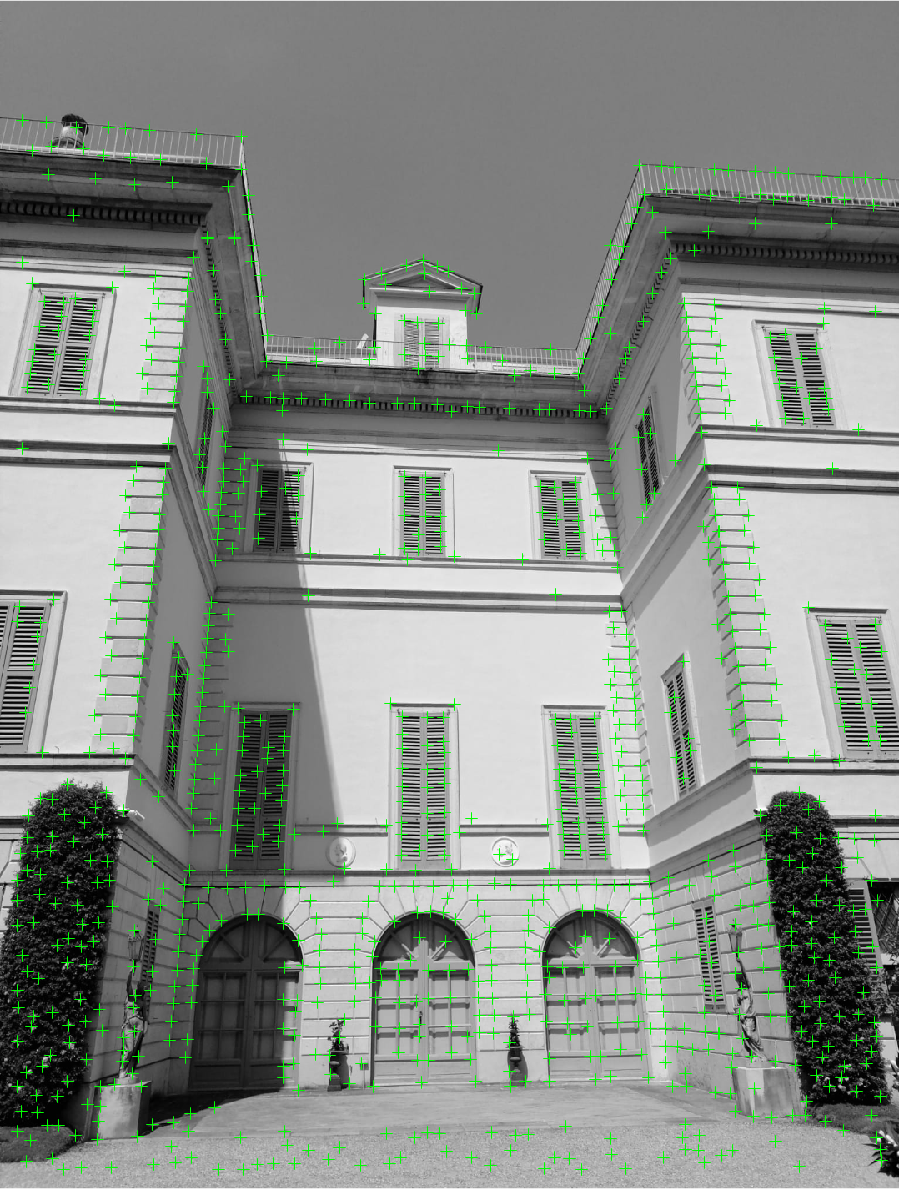
\includegraphics[width=0.45\linewidth]{image_corners.png}
	\captionof{figure}{Extracted corners of the image}
	\label{image_corners}
\end{figure*}


\section{2D reconstruction of a horizontal section}
\textbf{Rectify (2D reconstruct) the horizontal section of the building from the useful selected image lines and features, including vertical shadows. In particular, determine the ratio between the width of facade 2 (or 4) and the width of facade 3.} \hfill \break
We performed 2D reconstruction of the horizontal section of the building utilizing a stratified approach instead of a direct one in order to increase robustness (numerical errors should decrease). The stratified approach consists of performing sequentially an affine reconstruction and a shape reconstruction of the original image. We first computed the affine mapping $H_{affine}$ that maps the original image to its affine reconstruction. Then, we computed the similarity mapping $H_{shape}$ that maps the obtained affine reconstruction to its shape reconstruction. The overall mapping $H_{r}$ that maps the original image to its shape reconstruction can be computed as follows:
$$ H_{r} = H_{shape} * H_{affine} $$

\subsection{Affine reconstruction}
To compute $H_{affine}$ we exploited the fact that a projective mapping $H$ maps the line at the infinity $l_{\infty} = [0\quad0\quad1]^\intercal$ onto itself if and only if $H$ is affine. Thus, this mapping must map any point $x'$ belonging to	$l'_{\infty}$ (image of the $l_{\infty}$) onto a point at the infinity, namely:

\begin{equation}
	H_{affine} \; x' = 
	\begin{bmatrix}
		* \\ * \\ 0
	\end{bmatrix}
	\Rightarrow
	\begin{bmatrix}
		* & * & * \\ * & * & * \\ & {l'}^{\intercal}_{\infty} &
	\end{bmatrix}
	\: x' =
	\begin{bmatrix}
		* & * & * \\ * & * & * \\ & {l'}^{\intercal}_{\infty} \; x' &
	\end{bmatrix}
	=
	\begin{bmatrix}
		* \\ * \\ 0
	\end{bmatrix}
\end{equation}

Taking into account that $H_{affine}$ should have the previous form and be non-singular, we chose the following matrix representation (the simplest one):
\begin{equation}
	H_{affine} =
	\begin{bmatrix}
		1 & 0 & 0 \\ 0 & 1 & 0 \\ & {l'}^{\intercal}_{\infty} &
	\end{bmatrix}
\end{equation}

For the computation of the line at the infinity $l'_{\infty}$, we exploited the blue points highlighted in Fig. \ref{image_original_lines} (the green points were utilized in the shape reconstruction). First of all, we considered an horizontal plane parallel to the floor highlighting the blue point a, b, c and d. Afterwards, we computed the first vanishing point vp1 (not represented in the figure) as the intersection of the two lines ab and dc (images of parallel lines in the real scene), while the second vanishing point vp2 as the intersection of the two lines ad and bc (images of parallel lines in the real scene). Eventually, we computed $l'_{\infty}$ as the cross product of the two vanishing points (they belong to the image of the line at the infinity), obtaining the mapping $H_{affine}$ as previously stated.

The resulting affine reconstruction obtained applying $H_{affine}$ to the original image is shown in Fig. \ref{image_affine_reconstruction}.

\begin{figure}[!h]
	\centering
	\begin{minipage}{.45\textwidth}
		\centering
		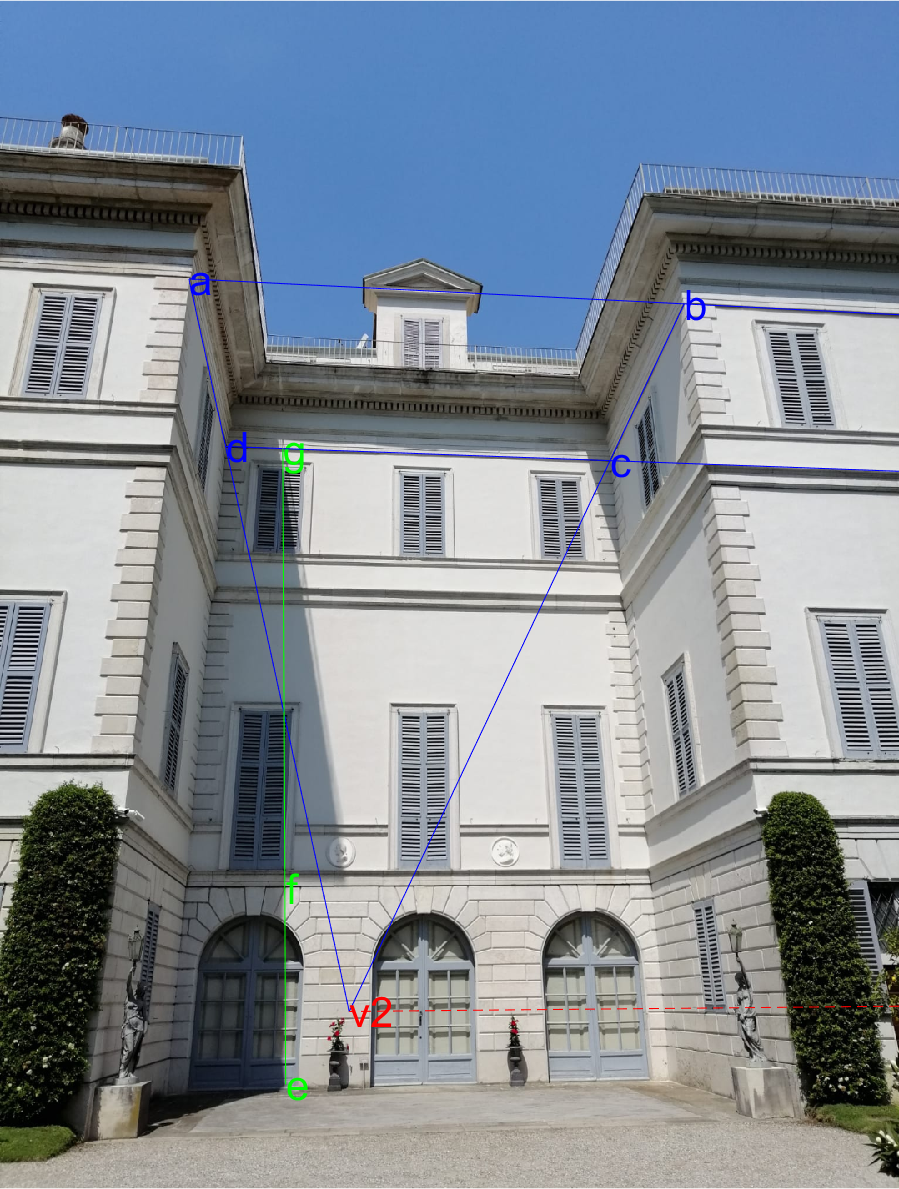
\includegraphics[scale = 0.4]{image_original_lines.png}
		\captionof{figure}{Features and lines in the original image used for affine and shape reconstruction}
		\label{image_original_lines}
	\end{minipage}%
	\begin{minipage}{.5\textwidth}
		\centering
		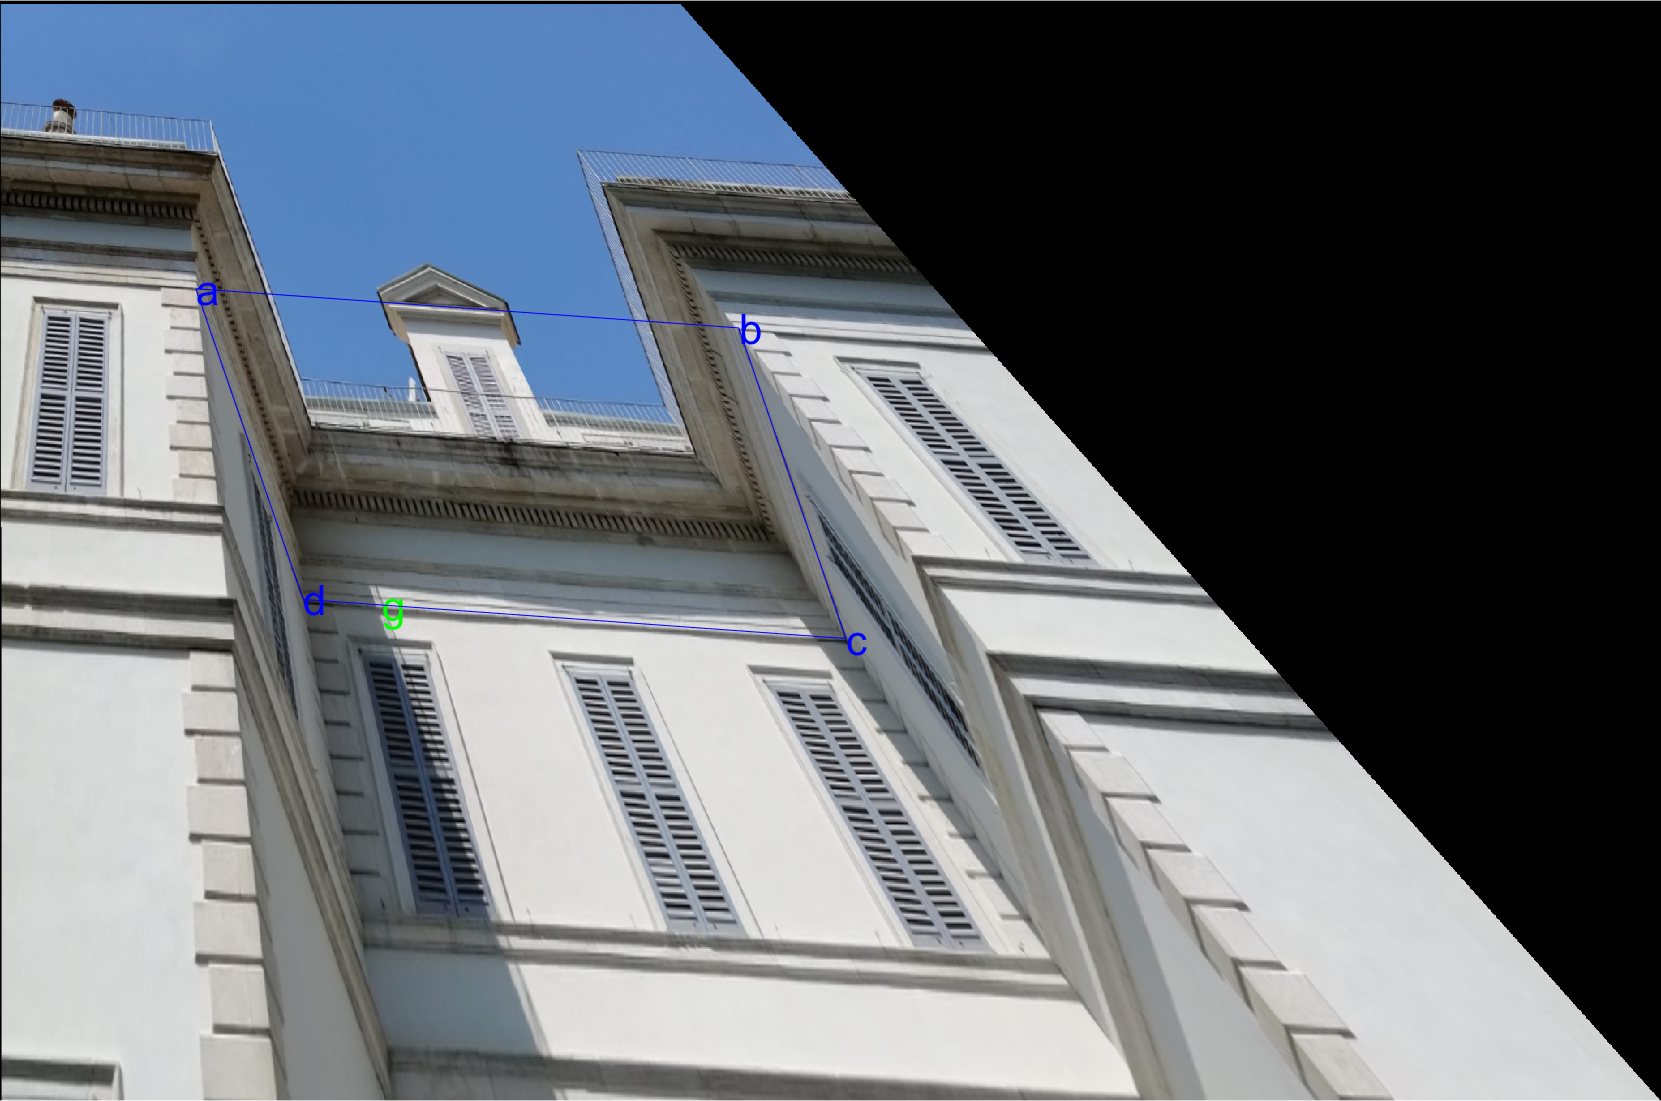
\includegraphics[scale = 0.3]{image_affine_reconstruction.png}
		\captionof{figure}{Affine reconstruction of the original image}
		\label{image_affine_reconstruction}
	\end{minipage}
\end{figure}

\begin{figure*}[!h]

\end{figure*}




\end{document}